% Created by tikzDevice version 0.12 on 2019-03-18 14:54:16
% !TEX encoding = UTF-8 Unicode
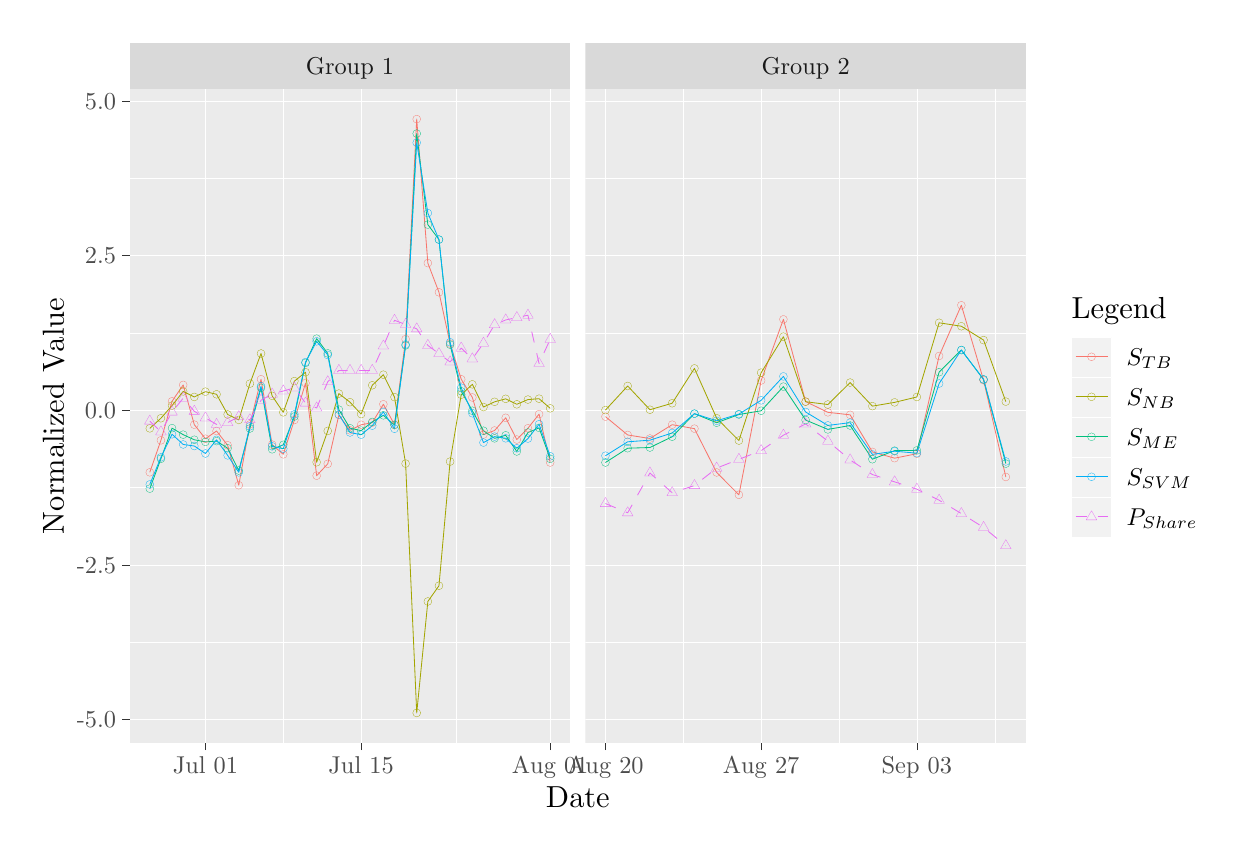
\begin{tikzpicture}[x=1pt,y=1pt]
\definecolor{fillColor}{RGB}{255,255,255}
\path[use as bounding box,fill=fillColor,fill opacity=0.00] (0,0) rectangle (433.62,289.08);
\begin{scope}
\path[clip] (  0.00,  0.00) rectangle (433.62,289.08);
\definecolor{drawColor}{RGB}{255,255,255}
\definecolor{fillColor}{RGB}{255,255,255}

\path[draw=drawColor,line width= 0.1pt,line join=round,line cap=round,fill=fillColor] (  0.00,  0.00) rectangle (433.62,289.08);
\end{scope}
\begin{scope}
\path[clip] ( 36.90, 30.73) rectangle (196.04,266.77);
\definecolor{fillColor}{gray}{0.92}

\path[fill=fillColor] ( 36.90, 30.73) rectangle (196.04,266.77);
\definecolor{drawColor}{RGB}{255,255,255}

\path[draw=drawColor,line width= 0.1pt,line join=round] ( 36.90, 67.00) --
	(196.04, 67.00);

\path[draw=drawColor,line width= 0.1pt,line join=round] ( 36.90,122.89) --
	(196.04,122.89);

\path[draw=drawColor,line width= 0.1pt,line join=round] ( 36.90,178.79) --
	(196.04,178.79);

\path[draw=drawColor,line width= 0.1pt,line join=round] ( 36.90,234.68) --
	(196.04,234.68);

\path[draw=drawColor,line width= 0.1pt,line join=round] ( 92.36, 30.73) --
	( 92.36,266.77);

\path[draw=drawColor,line width= 0.1pt,line join=round] (154.65, 30.73) --
	(154.65,266.77);

\path[draw=drawColor,line width= 0.1pt,line join=round] ( 36.90, 39.05) --
	(196.04, 39.05);

\path[draw=drawColor,line width= 0.1pt,line join=round] ( 36.90, 94.95) --
	(196.04, 94.95);

\path[draw=drawColor,line width= 0.1pt,line join=round] ( 36.90,150.84) --
	(196.04,150.84);

\path[draw=drawColor,line width= 0.1pt,line join=round] ( 36.90,206.73) --
	(196.04,206.73);

\path[draw=drawColor,line width= 0.1pt,line join=round] ( 36.90,262.63) --
	(196.04,262.63);

\path[draw=drawColor,line width= 0.1pt,line join=round] ( 64.23, 30.73) --
	( 64.23,266.77);

\path[draw=drawColor,line width= 0.1pt,line join=round] (120.49, 30.73) --
	(120.49,266.77);

\path[draw=drawColor,line width= 0.1pt,line join=round] (188.81, 30.73) --
	(188.81,266.77);
\definecolor{drawColor}{RGB}{248,118,109}

\path[draw=drawColor,line width= 0.3pt,line join=round] ( 44.13,128.42) --
	( 48.15,139.97) --
	( 52.17,154.07) --
	( 56.19,159.99) --
	( 60.21,145.63) --
	( 64.23,140.54) --
	( 68.25,143.33) --
	( 72.26,138.19) --
	( 76.28,123.74) --
	( 80.30,145.71) --
	( 84.32,162.05) --
	( 88.34,138.42) --
	( 92.36,134.91) --
	( 96.38,147.31) --
	(100.40,160.65) --
	(104.42,127.19) --
	(108.43,131.47) --
	(112.45,149.12) --
	(116.47,143.59) --
	(120.49,145.58) --
	(124.51,146.35) --
	(128.53,153.00) --
	(132.55,145.64) --
	(136.57,176.53) --
	(140.58,256.04) --
	(144.60,204.01) --
	(148.62,193.46) --
	(152.64,174.91) --
	(156.66,162.04) --
	(160.68,155.46) --
	(164.70,142.05) --
	(168.72,143.52) --
	(172.73,148.10) --
	(176.75,140.24) --
	(180.77,144.34) --
	(184.79,149.44) --
	(188.81,131.95);
\definecolor{drawColor}{RGB}{163,165,0}

\path[draw=drawColor,line width= 0.3pt,line join=round] ( 44.13,144.29) --
	( 48.15,147.95) --
	( 52.17,152.52) --
	( 56.19,157.64) --
	( 60.21,155.64) --
	( 64.23,157.55) --
	( 68.25,156.60) --
	( 72.26,149.32) --
	( 76.28,147.34) --
	( 80.30,160.45) --
	( 84.32,171.34) --
	( 88.34,156.03) --
	( 92.36,150.08) --
	( 96.38,161.36) --
	(100.40,164.58) --
	(104.42,132.05) --
	(108.43,143.36) --
	(112.45,156.86) --
	(116.47,153.75) --
	(120.49,149.45) --
	(124.51,159.86) --
	(128.53,163.69) --
	(132.55,155.58) --
	(136.57,131.56) --
	(140.58, 41.46) --
	(144.60, 81.74) --
	(148.62, 87.42) --
	(152.64,132.29) --
	(156.66,156.46) --
	(160.68,160.20) --
	(164.70,151.99) --
	(168.72,153.88) --
	(172.73,154.96) --
	(176.75,152.99) --
	(180.77,154.69) --
	(184.79,155.01) --
	(188.81,151.53);
\definecolor{drawColor}{RGB}{0,191,125}

\path[draw=drawColor,line width= 0.3pt,line join=round] ( 44.13,122.50) --
	( 48.15,133.29) --
	( 52.17,144.37) --
	( 56.19,142.01) --
	( 60.21,140.17) --
	( 64.23,139.40) --
	( 68.25,139.69) --
	( 72.26,137.11) --
	( 76.28,129.05) --
	( 80.30,144.24) --
	( 84.32,158.93) --
	( 88.34,136.73) --
	( 92.36,138.35) --
	( 96.38,148.58) --
	(100.40,167.95) --
	(104.42,176.71) --
	(108.43,171.39) --
	(112.45,151.05) --
	(116.47,144.35) --
	(120.49,143.47) --
	(124.51,146.61) --
	(128.53,149.00) --
	(132.55,145.50) --
	(136.57,174.28) --
	(140.58,250.81) --
	(144.60,217.91) --
	(148.62,212.52) --
	(152.64,174.52) --
	(156.66,157.70) --
	(160.68,150.66) --
	(164.70,143.43) --
	(168.72,140.68) --
	(172.73,141.78) --
	(176.75,135.94) --
	(180.77,142.79) --
	(184.79,144.46) --
	(188.81,133.28);
\definecolor{drawColor}{RGB}{0,176,246}

\path[draw=drawColor,line width= 0.3pt,line join=round] ( 44.13,124.04) --
	( 48.15,133.83) --
	( 52.17,142.17) --
	( 56.19,138.47) --
	( 60.21,137.91) --
	( 64.23,135.21) --
	( 68.25,140.14) --
	( 72.26,134.53) --
	( 76.28,128.40) --
	( 80.30,145.03) --
	( 84.32,159.51) --
	( 88.34,137.80) --
	( 92.36,136.92) --
	( 96.38,149.36) --
	(100.40,168.23) --
	(104.42,175.74) --
	(108.43,170.80) --
	(112.45,149.30) --
	(116.47,142.81) --
	(120.49,141.98) --
	(124.51,145.26) --
	(128.53,150.23) --
	(132.55,144.14) --
	(136.57,174.61) --
	(140.58,247.51) --
	(144.60,222.08) --
	(148.62,212.47) --
	(152.64,175.40) --
	(156.66,158.96) --
	(160.68,149.76) --
	(164.70,139.15) --
	(168.72,141.31) --
	(172.73,140.70) --
	(176.75,137.09) --
	(180.77,140.60) --
	(184.79,145.78) --
	(188.81,134.21);
\definecolor{drawColor}{RGB}{231,107,243}

\path[draw=drawColor,line width= 0.3pt,dash pattern=on 4pt off 4pt ,line join=round] ( 44.13,146.93) --
	( 48.15,143.03) --
	( 52.17,150.18) --
	( 56.19,155.19) --
	( 60.21,150.45) --
	( 64.23,148.09) --
	( 68.25,145.72) --
	( 72.26,146.37) --
	( 76.28,148.50) --
	( 80.30,147.39) --
	( 84.32,154.45) --
	( 88.34,156.68) --
	( 92.36,157.79) --
	( 96.38,158.90) --
	(100.40,153.43) --
	(104.42,151.66) --
	(108.43,161.13) --
	(112.45,165.22) --
	(116.47,165.22) --
	(120.49,165.22) --
	(124.51,165.22) --
	(128.53,174.04) --
	(132.55,183.33) --
	(136.57,181.84) --
	(140.58,180.26) --
	(144.60,174.27) --
	(148.62,171.28) --
	(152.64,168.28) --
	(156.66,173.30) --
	(160.68,169.40) --
	(164.70,175.06) --
	(168.72,181.75) --
	(172.73,183.46) --
	(176.75,184.32) --
	(180.77,185.18) --
	(184.79,167.73) --
	(188.81,176.45);
\definecolor{drawColor}{RGB}{248,118,109}

\path[draw=drawColor,line width= 0.1pt,line join=round,line cap=round] ( 44.13,128.42) circle (  1.43);

\path[draw=drawColor,line width= 0.1pt,line join=round,line cap=round] ( 48.15,139.97) circle (  1.43);

\path[draw=drawColor,line width= 0.1pt,line join=round,line cap=round] ( 52.17,154.07) circle (  1.43);

\path[draw=drawColor,line width= 0.1pt,line join=round,line cap=round] ( 56.19,159.99) circle (  1.43);

\path[draw=drawColor,line width= 0.1pt,line join=round,line cap=round] ( 60.21,145.63) circle (  1.43);

\path[draw=drawColor,line width= 0.1pt,line join=round,line cap=round] ( 64.23,140.54) circle (  1.43);

\path[draw=drawColor,line width= 0.1pt,line join=round,line cap=round] ( 68.25,143.33) circle (  1.43);

\path[draw=drawColor,line width= 0.1pt,line join=round,line cap=round] ( 72.26,138.19) circle (  1.43);

\path[draw=drawColor,line width= 0.1pt,line join=round,line cap=round] ( 76.28,123.74) circle (  1.43);

\path[draw=drawColor,line width= 0.1pt,line join=round,line cap=round] ( 80.30,145.71) circle (  1.43);

\path[draw=drawColor,line width= 0.1pt,line join=round,line cap=round] ( 84.32,162.05) circle (  1.43);

\path[draw=drawColor,line width= 0.1pt,line join=round,line cap=round] ( 88.34,138.42) circle (  1.43);

\path[draw=drawColor,line width= 0.1pt,line join=round,line cap=round] ( 92.36,134.91) circle (  1.43);

\path[draw=drawColor,line width= 0.1pt,line join=round,line cap=round] ( 96.38,147.31) circle (  1.43);

\path[draw=drawColor,line width= 0.1pt,line join=round,line cap=round] (100.40,160.65) circle (  1.43);

\path[draw=drawColor,line width= 0.1pt,line join=round,line cap=round] (104.42,127.19) circle (  1.43);

\path[draw=drawColor,line width= 0.1pt,line join=round,line cap=round] (108.43,131.47) circle (  1.43);

\path[draw=drawColor,line width= 0.1pt,line join=round,line cap=round] (112.45,149.12) circle (  1.43);

\path[draw=drawColor,line width= 0.1pt,line join=round,line cap=round] (116.47,143.59) circle (  1.43);

\path[draw=drawColor,line width= 0.1pt,line join=round,line cap=round] (120.49,145.58) circle (  1.43);

\path[draw=drawColor,line width= 0.1pt,line join=round,line cap=round] (124.51,146.35) circle (  1.43);

\path[draw=drawColor,line width= 0.1pt,line join=round,line cap=round] (128.53,153.00) circle (  1.43);

\path[draw=drawColor,line width= 0.1pt,line join=round,line cap=round] (132.55,145.64) circle (  1.43);

\path[draw=drawColor,line width= 0.1pt,line join=round,line cap=round] (136.57,176.53) circle (  1.43);

\path[draw=drawColor,line width= 0.1pt,line join=round,line cap=round] (140.58,256.04) circle (  1.43);

\path[draw=drawColor,line width= 0.1pt,line join=round,line cap=round] (144.60,204.01) circle (  1.43);

\path[draw=drawColor,line width= 0.1pt,line join=round,line cap=round] (148.62,193.46) circle (  1.43);

\path[draw=drawColor,line width= 0.1pt,line join=round,line cap=round] (152.64,174.91) circle (  1.43);

\path[draw=drawColor,line width= 0.1pt,line join=round,line cap=round] (156.66,162.04) circle (  1.43);

\path[draw=drawColor,line width= 0.1pt,line join=round,line cap=round] (160.68,155.46) circle (  1.43);

\path[draw=drawColor,line width= 0.1pt,line join=round,line cap=round] (164.70,142.05) circle (  1.43);

\path[draw=drawColor,line width= 0.1pt,line join=round,line cap=round] (168.72,143.52) circle (  1.43);

\path[draw=drawColor,line width= 0.1pt,line join=round,line cap=round] (172.73,148.10) circle (  1.43);

\path[draw=drawColor,line width= 0.1pt,line join=round,line cap=round] (176.75,140.24) circle (  1.43);

\path[draw=drawColor,line width= 0.1pt,line join=round,line cap=round] (180.77,144.34) circle (  1.43);

\path[draw=drawColor,line width= 0.1pt,line join=round,line cap=round] (184.79,149.44) circle (  1.43);

\path[draw=drawColor,line width= 0.1pt,line join=round,line cap=round] (188.81,131.95) circle (  1.43);
\definecolor{drawColor}{RGB}{163,165,0}

\path[draw=drawColor,line width= 0.1pt,line join=round,line cap=round] ( 44.13,144.29) circle (  1.43);

\path[draw=drawColor,line width= 0.1pt,line join=round,line cap=round] ( 48.15,147.95) circle (  1.43);

\path[draw=drawColor,line width= 0.1pt,line join=round,line cap=round] ( 52.17,152.52) circle (  1.43);

\path[draw=drawColor,line width= 0.1pt,line join=round,line cap=round] ( 56.19,157.64) circle (  1.43);

\path[draw=drawColor,line width= 0.1pt,line join=round,line cap=round] ( 60.21,155.64) circle (  1.43);

\path[draw=drawColor,line width= 0.1pt,line join=round,line cap=round] ( 64.23,157.55) circle (  1.43);

\path[draw=drawColor,line width= 0.1pt,line join=round,line cap=round] ( 68.25,156.60) circle (  1.43);

\path[draw=drawColor,line width= 0.1pt,line join=round,line cap=round] ( 72.26,149.32) circle (  1.43);

\path[draw=drawColor,line width= 0.1pt,line join=round,line cap=round] ( 76.28,147.34) circle (  1.43);

\path[draw=drawColor,line width= 0.1pt,line join=round,line cap=round] ( 80.30,160.45) circle (  1.43);

\path[draw=drawColor,line width= 0.1pt,line join=round,line cap=round] ( 84.32,171.34) circle (  1.43);

\path[draw=drawColor,line width= 0.1pt,line join=round,line cap=round] ( 88.34,156.03) circle (  1.43);

\path[draw=drawColor,line width= 0.1pt,line join=round,line cap=round] ( 92.36,150.08) circle (  1.43);

\path[draw=drawColor,line width= 0.1pt,line join=round,line cap=round] ( 96.38,161.36) circle (  1.43);

\path[draw=drawColor,line width= 0.1pt,line join=round,line cap=round] (100.40,164.58) circle (  1.43);

\path[draw=drawColor,line width= 0.1pt,line join=round,line cap=round] (104.42,132.05) circle (  1.43);

\path[draw=drawColor,line width= 0.1pt,line join=round,line cap=round] (108.43,143.36) circle (  1.43);

\path[draw=drawColor,line width= 0.1pt,line join=round,line cap=round] (112.45,156.86) circle (  1.43);

\path[draw=drawColor,line width= 0.1pt,line join=round,line cap=round] (116.47,153.75) circle (  1.43);

\path[draw=drawColor,line width= 0.1pt,line join=round,line cap=round] (120.49,149.45) circle (  1.43);

\path[draw=drawColor,line width= 0.1pt,line join=round,line cap=round] (124.51,159.86) circle (  1.43);

\path[draw=drawColor,line width= 0.1pt,line join=round,line cap=round] (128.53,163.69) circle (  1.43);

\path[draw=drawColor,line width= 0.1pt,line join=round,line cap=round] (132.55,155.58) circle (  1.43);

\path[draw=drawColor,line width= 0.1pt,line join=round,line cap=round] (136.57,131.56) circle (  1.43);

\path[draw=drawColor,line width= 0.1pt,line join=round,line cap=round] (140.58, 41.46) circle (  1.43);

\path[draw=drawColor,line width= 0.1pt,line join=round,line cap=round] (144.60, 81.74) circle (  1.43);

\path[draw=drawColor,line width= 0.1pt,line join=round,line cap=round] (148.62, 87.42) circle (  1.43);

\path[draw=drawColor,line width= 0.1pt,line join=round,line cap=round] (152.64,132.29) circle (  1.43);

\path[draw=drawColor,line width= 0.1pt,line join=round,line cap=round] (156.66,156.46) circle (  1.43);

\path[draw=drawColor,line width= 0.1pt,line join=round,line cap=round] (160.68,160.20) circle (  1.43);

\path[draw=drawColor,line width= 0.1pt,line join=round,line cap=round] (164.70,151.99) circle (  1.43);

\path[draw=drawColor,line width= 0.1pt,line join=round,line cap=round] (168.72,153.88) circle (  1.43);

\path[draw=drawColor,line width= 0.1pt,line join=round,line cap=round] (172.73,154.96) circle (  1.43);

\path[draw=drawColor,line width= 0.1pt,line join=round,line cap=round] (176.75,152.99) circle (  1.43);

\path[draw=drawColor,line width= 0.1pt,line join=round,line cap=round] (180.77,154.69) circle (  1.43);

\path[draw=drawColor,line width= 0.1pt,line join=round,line cap=round] (184.79,155.01) circle (  1.43);

\path[draw=drawColor,line width= 0.1pt,line join=round,line cap=round] (188.81,151.53) circle (  1.43);
\definecolor{drawColor}{RGB}{0,191,125}

\path[draw=drawColor,line width= 0.1pt,line join=round,line cap=round] ( 44.13,122.50) circle (  1.43);

\path[draw=drawColor,line width= 0.1pt,line join=round,line cap=round] ( 48.15,133.29) circle (  1.43);

\path[draw=drawColor,line width= 0.1pt,line join=round,line cap=round] ( 52.17,144.37) circle (  1.43);

\path[draw=drawColor,line width= 0.1pt,line join=round,line cap=round] ( 56.19,142.01) circle (  1.43);

\path[draw=drawColor,line width= 0.1pt,line join=round,line cap=round] ( 60.21,140.17) circle (  1.43);

\path[draw=drawColor,line width= 0.1pt,line join=round,line cap=round] ( 64.23,139.40) circle (  1.43);

\path[draw=drawColor,line width= 0.1pt,line join=round,line cap=round] ( 68.25,139.69) circle (  1.43);

\path[draw=drawColor,line width= 0.1pt,line join=round,line cap=round] ( 72.26,137.11) circle (  1.43);

\path[draw=drawColor,line width= 0.1pt,line join=round,line cap=round] ( 76.28,129.05) circle (  1.43);

\path[draw=drawColor,line width= 0.1pt,line join=round,line cap=round] ( 80.30,144.24) circle (  1.43);

\path[draw=drawColor,line width= 0.1pt,line join=round,line cap=round] ( 84.32,158.93) circle (  1.43);

\path[draw=drawColor,line width= 0.1pt,line join=round,line cap=round] ( 88.34,136.73) circle (  1.43);

\path[draw=drawColor,line width= 0.1pt,line join=round,line cap=round] ( 92.36,138.35) circle (  1.43);

\path[draw=drawColor,line width= 0.1pt,line join=round,line cap=round] ( 96.38,148.58) circle (  1.43);

\path[draw=drawColor,line width= 0.1pt,line join=round,line cap=round] (100.40,167.95) circle (  1.43);

\path[draw=drawColor,line width= 0.1pt,line join=round,line cap=round] (104.42,176.71) circle (  1.43);

\path[draw=drawColor,line width= 0.1pt,line join=round,line cap=round] (108.43,171.39) circle (  1.43);

\path[draw=drawColor,line width= 0.1pt,line join=round,line cap=round] (112.45,151.05) circle (  1.43);

\path[draw=drawColor,line width= 0.1pt,line join=round,line cap=round] (116.47,144.35) circle (  1.43);

\path[draw=drawColor,line width= 0.1pt,line join=round,line cap=round] (120.49,143.47) circle (  1.43);

\path[draw=drawColor,line width= 0.1pt,line join=round,line cap=round] (124.51,146.61) circle (  1.43);

\path[draw=drawColor,line width= 0.1pt,line join=round,line cap=round] (128.53,149.00) circle (  1.43);

\path[draw=drawColor,line width= 0.1pt,line join=round,line cap=round] (132.55,145.50) circle (  1.43);

\path[draw=drawColor,line width= 0.1pt,line join=round,line cap=round] (136.57,174.28) circle (  1.43);

\path[draw=drawColor,line width= 0.1pt,line join=round,line cap=round] (140.58,250.81) circle (  1.43);

\path[draw=drawColor,line width= 0.1pt,line join=round,line cap=round] (144.60,217.91) circle (  1.43);

\path[draw=drawColor,line width= 0.1pt,line join=round,line cap=round] (148.62,212.52) circle (  1.43);

\path[draw=drawColor,line width= 0.1pt,line join=round,line cap=round] (152.64,174.52) circle (  1.43);

\path[draw=drawColor,line width= 0.1pt,line join=round,line cap=round] (156.66,157.70) circle (  1.43);

\path[draw=drawColor,line width= 0.1pt,line join=round,line cap=round] (160.68,150.66) circle (  1.43);

\path[draw=drawColor,line width= 0.1pt,line join=round,line cap=round] (164.70,143.43) circle (  1.43);

\path[draw=drawColor,line width= 0.1pt,line join=round,line cap=round] (168.72,140.68) circle (  1.43);

\path[draw=drawColor,line width= 0.1pt,line join=round,line cap=round] (172.73,141.78) circle (  1.43);

\path[draw=drawColor,line width= 0.1pt,line join=round,line cap=round] (176.75,135.94) circle (  1.43);

\path[draw=drawColor,line width= 0.1pt,line join=round,line cap=round] (180.77,142.79) circle (  1.43);

\path[draw=drawColor,line width= 0.1pt,line join=round,line cap=round] (184.79,144.46) circle (  1.43);

\path[draw=drawColor,line width= 0.1pt,line join=round,line cap=round] (188.81,133.28) circle (  1.43);
\definecolor{drawColor}{RGB}{0,176,246}

\path[draw=drawColor,line width= 0.1pt,line join=round,line cap=round] ( 44.13,124.04) circle (  1.43);

\path[draw=drawColor,line width= 0.1pt,line join=round,line cap=round] ( 48.15,133.83) circle (  1.43);

\path[draw=drawColor,line width= 0.1pt,line join=round,line cap=round] ( 52.17,142.17) circle (  1.43);

\path[draw=drawColor,line width= 0.1pt,line join=round,line cap=round] ( 56.19,138.47) circle (  1.43);

\path[draw=drawColor,line width= 0.1pt,line join=round,line cap=round] ( 60.21,137.91) circle (  1.43);

\path[draw=drawColor,line width= 0.1pt,line join=round,line cap=round] ( 64.23,135.21) circle (  1.43);

\path[draw=drawColor,line width= 0.1pt,line join=round,line cap=round] ( 68.25,140.14) circle (  1.43);

\path[draw=drawColor,line width= 0.1pt,line join=round,line cap=round] ( 72.26,134.53) circle (  1.43);

\path[draw=drawColor,line width= 0.1pt,line join=round,line cap=round] ( 76.28,128.40) circle (  1.43);

\path[draw=drawColor,line width= 0.1pt,line join=round,line cap=round] ( 80.30,145.03) circle (  1.43);

\path[draw=drawColor,line width= 0.1pt,line join=round,line cap=round] ( 84.32,159.51) circle (  1.43);

\path[draw=drawColor,line width= 0.1pt,line join=round,line cap=round] ( 88.34,137.80) circle (  1.43);

\path[draw=drawColor,line width= 0.1pt,line join=round,line cap=round] ( 92.36,136.92) circle (  1.43);

\path[draw=drawColor,line width= 0.1pt,line join=round,line cap=round] ( 96.38,149.36) circle (  1.43);

\path[draw=drawColor,line width= 0.1pt,line join=round,line cap=round] (100.40,168.23) circle (  1.43);

\path[draw=drawColor,line width= 0.1pt,line join=round,line cap=round] (104.42,175.74) circle (  1.43);

\path[draw=drawColor,line width= 0.1pt,line join=round,line cap=round] (108.43,170.80) circle (  1.43);

\path[draw=drawColor,line width= 0.1pt,line join=round,line cap=round] (112.45,149.30) circle (  1.43);

\path[draw=drawColor,line width= 0.1pt,line join=round,line cap=round] (116.47,142.81) circle (  1.43);

\path[draw=drawColor,line width= 0.1pt,line join=round,line cap=round] (120.49,141.98) circle (  1.43);

\path[draw=drawColor,line width= 0.1pt,line join=round,line cap=round] (124.51,145.26) circle (  1.43);

\path[draw=drawColor,line width= 0.1pt,line join=round,line cap=round] (128.53,150.23) circle (  1.43);

\path[draw=drawColor,line width= 0.1pt,line join=round,line cap=round] (132.55,144.14) circle (  1.43);

\path[draw=drawColor,line width= 0.1pt,line join=round,line cap=round] (136.57,174.61) circle (  1.43);

\path[draw=drawColor,line width= 0.1pt,line join=round,line cap=round] (140.58,247.51) circle (  1.43);

\path[draw=drawColor,line width= 0.1pt,line join=round,line cap=round] (144.60,222.08) circle (  1.43);

\path[draw=drawColor,line width= 0.1pt,line join=round,line cap=round] (148.62,212.47) circle (  1.43);

\path[draw=drawColor,line width= 0.1pt,line join=round,line cap=round] (152.64,175.40) circle (  1.43);

\path[draw=drawColor,line width= 0.1pt,line join=round,line cap=round] (156.66,158.96) circle (  1.43);

\path[draw=drawColor,line width= 0.1pt,line join=round,line cap=round] (160.68,149.76) circle (  1.43);

\path[draw=drawColor,line width= 0.1pt,line join=round,line cap=round] (164.70,139.15) circle (  1.43);

\path[draw=drawColor,line width= 0.1pt,line join=round,line cap=round] (168.72,141.31) circle (  1.43);

\path[draw=drawColor,line width= 0.1pt,line join=round,line cap=round] (172.73,140.70) circle (  1.43);

\path[draw=drawColor,line width= 0.1pt,line join=round,line cap=round] (176.75,137.09) circle (  1.43);

\path[draw=drawColor,line width= 0.1pt,line join=round,line cap=round] (180.77,140.60) circle (  1.43);

\path[draw=drawColor,line width= 0.1pt,line join=round,line cap=round] (184.79,145.78) circle (  1.43);

\path[draw=drawColor,line width= 0.1pt,line join=round,line cap=round] (188.81,134.21) circle (  1.43);
\definecolor{drawColor}{RGB}{231,107,243}

\path[draw=drawColor,line width= 0.1pt,line join=round,line cap=round] ( 44.13,149.14) --
	( 46.06,145.82) --
	( 42.21,145.82) --
	( 44.13,149.14);

\path[draw=drawColor,line width= 0.1pt,line join=round,line cap=round] ( 48.15,145.24) --
	( 50.07,141.92) --
	( 46.23,141.92) --
	( 48.15,145.24);

\path[draw=drawColor,line width= 0.1pt,line join=round,line cap=round] ( 52.17,152.39) --
	( 54.09,149.07) --
	( 50.25,149.07) --
	( 52.17,152.39);

\path[draw=drawColor,line width= 0.1pt,line join=round,line cap=round] ( 56.19,157.41) --
	( 58.11,154.08) --
	( 54.27,154.08) --
	( 56.19,157.41);

\path[draw=drawColor,line width= 0.1pt,line join=round,line cap=round] ( 60.21,152.67) --
	( 62.13,149.34) --
	( 58.29,149.34) --
	( 60.21,152.67);

\path[draw=drawColor,line width= 0.1pt,line join=round,line cap=round] ( 64.23,150.30) --
	( 66.15,146.98) --
	( 62.31,146.98) --
	( 64.23,150.30);

\path[draw=drawColor,line width= 0.1pt,line join=round,line cap=round] ( 68.25,147.94) --
	( 70.17,144.61) --
	( 66.32,144.61) --
	( 68.25,147.94);

\path[draw=drawColor,line width= 0.1pt,line join=round,line cap=round] ( 72.26,148.59) --
	( 74.19,145.26) --
	( 70.34,145.26) --
	( 72.26,148.59);

\path[draw=drawColor,line width= 0.1pt,line join=round,line cap=round] ( 76.28,150.72) --
	( 78.21,147.39) --
	( 74.36,147.39) --
	( 76.28,150.72);

\path[draw=drawColor,line width= 0.1pt,line join=round,line cap=round] ( 80.30,149.61) --
	( 82.22,146.28) --
	( 78.38,146.28) --
	( 80.30,149.61);

\path[draw=drawColor,line width= 0.1pt,line join=round,line cap=round] ( 84.32,156.67) --
	( 86.24,153.34) --
	( 82.40,153.34) --
	( 84.32,156.67);

\path[draw=drawColor,line width= 0.1pt,line join=round,line cap=round] ( 88.34,158.89) --
	( 90.26,155.57) --
	( 86.42,155.57) --
	( 88.34,158.89);

\path[draw=drawColor,line width= 0.1pt,line join=round,line cap=round] ( 92.36,160.01) --
	( 94.28,156.68) --
	( 90.44,156.68) --
	( 92.36,160.01);

\path[draw=drawColor,line width= 0.1pt,line join=round,line cap=round] ( 96.38,161.12) --
	( 98.30,157.79) --
	( 94.46,157.79) --
	( 96.38,161.12);

\path[draw=drawColor,line width= 0.1pt,line join=round,line cap=round] (100.40,155.64) --
	(102.32,152.32) --
	( 98.47,152.32) --
	(100.40,155.64);

\path[draw=drawColor,line width= 0.1pt,line join=round,line cap=round] (104.42,153.88) --
	(106.34,150.55) --
	(102.49,150.55) --
	(104.42,153.88);

\path[draw=drawColor,line width= 0.1pt,line join=round,line cap=round] (108.43,163.35) --
	(110.36,160.02) --
	(106.51,160.02) --
	(108.43,163.35);

\path[draw=drawColor,line width= 0.1pt,line join=round,line cap=round] (112.45,167.44) --
	(114.37,164.11) --
	(110.53,164.11) --
	(112.45,167.44);

\path[draw=drawColor,line width= 0.1pt,line join=round,line cap=round] (116.47,167.44) --
	(118.39,164.11) --
	(114.55,164.11) --
	(116.47,167.44);

\path[draw=drawColor,line width= 0.1pt,line join=round,line cap=round] (120.49,167.44) --
	(122.41,164.11) --
	(118.57,164.11) --
	(120.49,167.44);

\path[draw=drawColor,line width= 0.1pt,line join=round,line cap=round] (124.51,167.44) --
	(126.43,164.11) --
	(122.59,164.11) --
	(124.51,167.44);

\path[draw=drawColor,line width= 0.1pt,line join=round,line cap=round] (128.53,176.26) --
	(130.45,172.93) --
	(126.61,172.93) --
	(128.53,176.26);

\path[draw=drawColor,line width= 0.1pt,line join=round,line cap=round] (132.55,185.54) --
	(134.47,182.22) --
	(130.62,182.22) --
	(132.55,185.54);

\path[draw=drawColor,line width= 0.1pt,line join=round,line cap=round] (136.57,184.06) --
	(138.49,180.73) --
	(134.64,180.73) --
	(136.57,184.06);

\path[draw=drawColor,line width= 0.1pt,line join=round,line cap=round] (140.58,182.48) --
	(142.51,179.15) --
	(138.66,179.15) --
	(140.58,182.48);

\path[draw=drawColor,line width= 0.1pt,line join=round,line cap=round] (144.60,176.49) --
	(146.52,173.16) --
	(142.68,173.16) --
	(144.60,176.49);

\path[draw=drawColor,line width= 0.1pt,line join=round,line cap=round] (148.62,173.50) --
	(150.54,170.17) --
	(146.70,170.17) --
	(148.62,173.50);

\path[draw=drawColor,line width= 0.1pt,line join=round,line cap=round] (152.64,170.50) --
	(154.56,167.17) --
	(150.72,167.17) --
	(152.64,170.50);

\path[draw=drawColor,line width= 0.1pt,line join=round,line cap=round] (156.66,175.52) --
	(158.58,172.19) --
	(154.74,172.19) --
	(156.66,175.52);

\path[draw=drawColor,line width= 0.1pt,line join=round,line cap=round] (160.68,171.62) --
	(162.60,168.29) --
	(158.76,168.29) --
	(160.68,171.62);

\path[draw=drawColor,line width= 0.1pt,line join=round,line cap=round] (164.70,177.28) --
	(166.62,173.95) --
	(162.78,173.95) --
	(164.70,177.28);

\path[draw=drawColor,line width= 0.1pt,line join=round,line cap=round] (168.72,183.97) --
	(170.64,180.64) --
	(166.79,180.64) --
	(168.72,183.97);

\path[draw=drawColor,line width= 0.1pt,line join=round,line cap=round] (172.73,185.68) --
	(174.66,182.36) --
	(170.81,182.36) --
	(172.73,185.68);

\path[draw=drawColor,line width= 0.1pt,line join=round,line cap=round] (176.75,186.54) --
	(178.67,183.21) --
	(174.83,183.21) --
	(176.75,186.54);

\path[draw=drawColor,line width= 0.1pt,line join=round,line cap=round] (180.77,187.40) --
	(182.69,184.07) --
	(178.85,184.07) --
	(180.77,187.40);

\path[draw=drawColor,line width= 0.1pt,line join=round,line cap=round] (184.79,169.94) --
	(186.71,166.62) --
	(182.87,166.62) --
	(184.79,169.94);

\path[draw=drawColor,line width= 0.1pt,line join=round,line cap=round] (188.81,178.67) --
	(190.73,175.34) --
	(186.89,175.34) --
	(188.81,178.67);
\end{scope}
\begin{scope}
\path[clip] (201.54, 30.73) rectangle (360.69,266.77);
\definecolor{fillColor}{gray}{0.92}

\path[fill=fillColor] (201.54, 30.73) rectangle (360.69,266.77);
\definecolor{drawColor}{RGB}{255,255,255}

\path[draw=drawColor,line width= 0.1pt,line join=round] (201.54, 67.00) --
	(360.69, 67.00);

\path[draw=drawColor,line width= 0.1pt,line join=round] (201.54,122.89) --
	(360.69,122.89);

\path[draw=drawColor,line width= 0.1pt,line join=round] (201.54,178.79) --
	(360.69,178.79);

\path[draw=drawColor,line width= 0.1pt,line join=round] (201.54,234.68) --
	(360.69,234.68);

\path[draw=drawColor,line width= 0.1pt,line join=round] (236.91, 30.73) --
	(236.91,266.77);

\path[draw=drawColor,line width= 0.1pt,line join=round] (293.17, 30.73) --
	(293.17,266.77);

\path[draw=drawColor,line width= 0.1pt,line join=round] (349.43, 30.73) --
	(349.43,266.77);

\path[draw=drawColor,line width= 0.1pt,line join=round] (201.54, 39.05) --
	(360.69, 39.05);

\path[draw=drawColor,line width= 0.1pt,line join=round] (201.54, 94.95) --
	(360.69, 94.95);

\path[draw=drawColor,line width= 0.1pt,line join=round] (201.54,150.84) --
	(360.69,150.84);

\path[draw=drawColor,line width= 0.1pt,line join=round] (201.54,206.73) --
	(360.69,206.73);

\path[draw=drawColor,line width= 0.1pt,line join=round] (201.54,262.63) --
	(360.69,262.63);

\path[draw=drawColor,line width= 0.1pt,line join=round] (208.78, 30.73) --
	(208.78,266.77);

\path[draw=drawColor,line width= 0.1pt,line join=round] (265.04, 30.73) --
	(265.04,266.77);

\path[draw=drawColor,line width= 0.1pt,line join=round] (321.30, 30.73) --
	(321.30,266.77);
\definecolor{drawColor}{RGB}{248,118,109}

\path[draw=drawColor,line width= 0.3pt,line join=round] (208.78,148.53) --
	(216.81,141.90) --
	(224.85,140.62) --
	(232.89,145.62) --
	(240.93,144.19) --
	(248.96,128.36) --
	(257.00,120.27) --
	(265.04,161.61) --
	(273.08,183.68) --
	(281.11,153.97) --
	(289.15,150.08) --
	(297.19,149.18) --
	(305.23,135.78) --
	(313.26,133.52) --
	(321.30,135.12) --
	(329.34,170.45) --
	(337.38,188.77) --
	(345.41,161.68) --
	(353.45,126.72);
\definecolor{drawColor}{RGB}{163,165,0}

\path[draw=drawColor,line width= 0.3pt,line join=round] (208.78,150.90) --
	(216.81,159.60) --
	(224.85,151.02) --
	(232.89,153.37) --
	(240.93,165.96) --
	(248.96,147.96) --
	(257.00,139.88) --
	(265.04,164.41) --
	(273.08,177.42) --
	(281.11,153.92) --
	(289.15,152.90) --
	(297.19,160.84) --
	(305.23,152.32) --
	(313.26,153.68) --
	(321.30,155.63) --
	(329.34,182.44) --
	(337.38,181.19) --
	(345.41,176.19) --
	(353.45,153.95);
\definecolor{drawColor}{RGB}{0,191,125}

\path[draw=drawColor,line width= 0.3pt,line join=round] (208.78,131.96) --
	(216.81,137.12) --
	(224.85,137.37) --
	(232.89,141.27) --
	(240.93,149.60) --
	(248.96,146.32) --
	(257.00,149.29) --
	(265.04,150.64) --
	(273.08,159.37) --
	(281.11,147.30) --
	(289.15,143.91) --
	(297.19,145.32) --
	(305.23,133.14) --
	(313.26,136.24) --
	(321.30,136.33) --
	(329.34,164.58) --
	(337.38,172.61) --
	(345.41,161.95) --
	(353.45,131.55);
\definecolor{drawColor}{RGB}{0,176,246}

\path[draw=drawColor,line width= 0.3pt,line join=round] (208.78,134.40) --
	(216.81,139.44) --
	(224.85,140.02) --
	(232.89,142.62) --
	(240.93,149.61) --
	(248.96,147.02) --
	(257.00,149.45) --
	(265.04,154.43) --
	(273.08,163.07) --
	(281.11,150.21) --
	(289.15,145.35) --
	(297.19,146.35) --
	(305.23,134.88) --
	(313.26,136.03) --
	(321.30,135.33) --
	(329.34,160.49) --
	(337.38,172.58) --
	(345.41,162.00) --
	(353.45,132.34);
\definecolor{drawColor}{RGB}{231,107,243}

\path[draw=drawColor,line width= 0.3pt,dash pattern=on 4pt off 4pt ,line join=round] (208.78,117.12) --
	(216.81,113.78) --
	(224.85,128.17) --
	(232.89,121.02) --
	(240.93,123.62) --
	(248.96,129.93) --
	(257.00,133.09) --
	(265.04,136.25) --
	(273.08,141.82) --
	(281.11,145.90) --
	(289.15,139.68) --
	(297.19,132.90) --
	(305.23,127.61) --
	(313.26,124.96) --
	(321.30,122.32) --
	(329.34,118.33) --
	(337.38,113.50) --
	(345.41,108.48) --
	(353.45,101.89);
\definecolor{drawColor}{RGB}{248,118,109}

\path[draw=drawColor,line width= 0.1pt,line join=round,line cap=round] (208.78,148.53) circle (  1.43);

\path[draw=drawColor,line width= 0.1pt,line join=round,line cap=round] (216.81,141.90) circle (  1.43);

\path[draw=drawColor,line width= 0.1pt,line join=round,line cap=round] (224.85,140.62) circle (  1.43);

\path[draw=drawColor,line width= 0.1pt,line join=round,line cap=round] (232.89,145.62) circle (  1.43);

\path[draw=drawColor,line width= 0.1pt,line join=round,line cap=round] (240.93,144.19) circle (  1.43);

\path[draw=drawColor,line width= 0.1pt,line join=round,line cap=round] (248.96,128.36) circle (  1.43);

\path[draw=drawColor,line width= 0.1pt,line join=round,line cap=round] (257.00,120.27) circle (  1.43);

\path[draw=drawColor,line width= 0.1pt,line join=round,line cap=round] (265.04,161.61) circle (  1.43);

\path[draw=drawColor,line width= 0.1pt,line join=round,line cap=round] (273.08,183.68) circle (  1.43);

\path[draw=drawColor,line width= 0.1pt,line join=round,line cap=round] (281.11,153.97) circle (  1.43);

\path[draw=drawColor,line width= 0.1pt,line join=round,line cap=round] (289.15,150.08) circle (  1.43);

\path[draw=drawColor,line width= 0.1pt,line join=round,line cap=round] (297.19,149.18) circle (  1.43);

\path[draw=drawColor,line width= 0.1pt,line join=round,line cap=round] (305.23,135.78) circle (  1.43);

\path[draw=drawColor,line width= 0.1pt,line join=round,line cap=round] (313.26,133.52) circle (  1.43);

\path[draw=drawColor,line width= 0.1pt,line join=round,line cap=round] (321.30,135.12) circle (  1.43);

\path[draw=drawColor,line width= 0.1pt,line join=round,line cap=round] (329.34,170.45) circle (  1.43);

\path[draw=drawColor,line width= 0.1pt,line join=round,line cap=round] (337.38,188.77) circle (  1.43);

\path[draw=drawColor,line width= 0.1pt,line join=round,line cap=round] (345.41,161.68) circle (  1.43);

\path[draw=drawColor,line width= 0.1pt,line join=round,line cap=round] (353.45,126.72) circle (  1.43);
\definecolor{drawColor}{RGB}{163,165,0}

\path[draw=drawColor,line width= 0.1pt,line join=round,line cap=round] (208.78,150.90) circle (  1.43);

\path[draw=drawColor,line width= 0.1pt,line join=round,line cap=round] (216.81,159.60) circle (  1.43);

\path[draw=drawColor,line width= 0.1pt,line join=round,line cap=round] (224.85,151.02) circle (  1.43);

\path[draw=drawColor,line width= 0.1pt,line join=round,line cap=round] (232.89,153.37) circle (  1.43);

\path[draw=drawColor,line width= 0.1pt,line join=round,line cap=round] (240.93,165.96) circle (  1.43);

\path[draw=drawColor,line width= 0.1pt,line join=round,line cap=round] (248.96,147.96) circle (  1.43);

\path[draw=drawColor,line width= 0.1pt,line join=round,line cap=round] (257.00,139.88) circle (  1.43);

\path[draw=drawColor,line width= 0.1pt,line join=round,line cap=round] (265.04,164.41) circle (  1.43);

\path[draw=drawColor,line width= 0.1pt,line join=round,line cap=round] (273.08,177.42) circle (  1.43);

\path[draw=drawColor,line width= 0.1pt,line join=round,line cap=round] (281.11,153.92) circle (  1.43);

\path[draw=drawColor,line width= 0.1pt,line join=round,line cap=round] (289.15,152.90) circle (  1.43);

\path[draw=drawColor,line width= 0.1pt,line join=round,line cap=round] (297.19,160.84) circle (  1.43);

\path[draw=drawColor,line width= 0.1pt,line join=round,line cap=round] (305.23,152.32) circle (  1.43);

\path[draw=drawColor,line width= 0.1pt,line join=round,line cap=round] (313.26,153.68) circle (  1.43);

\path[draw=drawColor,line width= 0.1pt,line join=round,line cap=round] (321.30,155.63) circle (  1.43);

\path[draw=drawColor,line width= 0.1pt,line join=round,line cap=round] (329.34,182.44) circle (  1.43);

\path[draw=drawColor,line width= 0.1pt,line join=round,line cap=round] (337.38,181.19) circle (  1.43);

\path[draw=drawColor,line width= 0.1pt,line join=round,line cap=round] (345.41,176.19) circle (  1.43);

\path[draw=drawColor,line width= 0.1pt,line join=round,line cap=round] (353.45,153.95) circle (  1.43);
\definecolor{drawColor}{RGB}{0,191,125}

\path[draw=drawColor,line width= 0.1pt,line join=round,line cap=round] (208.78,131.96) circle (  1.43);

\path[draw=drawColor,line width= 0.1pt,line join=round,line cap=round] (216.81,137.12) circle (  1.43);

\path[draw=drawColor,line width= 0.1pt,line join=round,line cap=round] (224.85,137.37) circle (  1.43);

\path[draw=drawColor,line width= 0.1pt,line join=round,line cap=round] (232.89,141.27) circle (  1.43);

\path[draw=drawColor,line width= 0.1pt,line join=round,line cap=round] (240.93,149.60) circle (  1.43);

\path[draw=drawColor,line width= 0.1pt,line join=round,line cap=round] (248.96,146.32) circle (  1.43);

\path[draw=drawColor,line width= 0.1pt,line join=round,line cap=round] (257.00,149.29) circle (  1.43);

\path[draw=drawColor,line width= 0.1pt,line join=round,line cap=round] (265.04,150.64) circle (  1.43);

\path[draw=drawColor,line width= 0.1pt,line join=round,line cap=round] (273.08,159.37) circle (  1.43);

\path[draw=drawColor,line width= 0.1pt,line join=round,line cap=round] (281.11,147.30) circle (  1.43);

\path[draw=drawColor,line width= 0.1pt,line join=round,line cap=round] (289.15,143.91) circle (  1.43);

\path[draw=drawColor,line width= 0.1pt,line join=round,line cap=round] (297.19,145.32) circle (  1.43);

\path[draw=drawColor,line width= 0.1pt,line join=round,line cap=round] (305.23,133.14) circle (  1.43);

\path[draw=drawColor,line width= 0.1pt,line join=round,line cap=round] (313.26,136.24) circle (  1.43);

\path[draw=drawColor,line width= 0.1pt,line join=round,line cap=round] (321.30,136.33) circle (  1.43);

\path[draw=drawColor,line width= 0.1pt,line join=round,line cap=round] (329.34,164.58) circle (  1.43);

\path[draw=drawColor,line width= 0.1pt,line join=round,line cap=round] (337.38,172.61) circle (  1.43);

\path[draw=drawColor,line width= 0.1pt,line join=round,line cap=round] (345.41,161.95) circle (  1.43);

\path[draw=drawColor,line width= 0.1pt,line join=round,line cap=round] (353.45,131.55) circle (  1.43);
\definecolor{drawColor}{RGB}{0,176,246}

\path[draw=drawColor,line width= 0.1pt,line join=round,line cap=round] (208.78,134.40) circle (  1.43);

\path[draw=drawColor,line width= 0.1pt,line join=round,line cap=round] (216.81,139.44) circle (  1.43);

\path[draw=drawColor,line width= 0.1pt,line join=round,line cap=round] (224.85,140.02) circle (  1.43);

\path[draw=drawColor,line width= 0.1pt,line join=round,line cap=round] (232.89,142.62) circle (  1.43);

\path[draw=drawColor,line width= 0.1pt,line join=round,line cap=round] (240.93,149.61) circle (  1.43);

\path[draw=drawColor,line width= 0.1pt,line join=round,line cap=round] (248.96,147.02) circle (  1.43);

\path[draw=drawColor,line width= 0.1pt,line join=round,line cap=round] (257.00,149.45) circle (  1.43);

\path[draw=drawColor,line width= 0.1pt,line join=round,line cap=round] (265.04,154.43) circle (  1.43);

\path[draw=drawColor,line width= 0.1pt,line join=round,line cap=round] (273.08,163.07) circle (  1.43);

\path[draw=drawColor,line width= 0.1pt,line join=round,line cap=round] (281.11,150.21) circle (  1.43);

\path[draw=drawColor,line width= 0.1pt,line join=round,line cap=round] (289.15,145.35) circle (  1.43);

\path[draw=drawColor,line width= 0.1pt,line join=round,line cap=round] (297.19,146.35) circle (  1.43);

\path[draw=drawColor,line width= 0.1pt,line join=round,line cap=round] (305.23,134.88) circle (  1.43);

\path[draw=drawColor,line width= 0.1pt,line join=round,line cap=round] (313.26,136.03) circle (  1.43);

\path[draw=drawColor,line width= 0.1pt,line join=round,line cap=round] (321.30,135.33) circle (  1.43);

\path[draw=drawColor,line width= 0.1pt,line join=round,line cap=round] (329.34,160.49) circle (  1.43);

\path[draw=drawColor,line width= 0.1pt,line join=round,line cap=round] (337.38,172.58) circle (  1.43);

\path[draw=drawColor,line width= 0.1pt,line join=round,line cap=round] (345.41,162.00) circle (  1.43);

\path[draw=drawColor,line width= 0.1pt,line join=round,line cap=round] (353.45,132.34) circle (  1.43);
\definecolor{drawColor}{RGB}{231,107,243}

\path[draw=drawColor,line width= 0.1pt,line join=round,line cap=round] (208.78,119.34) --
	(210.70,116.01) --
	(206.86,116.01) --
	(208.78,119.34);

\path[draw=drawColor,line width= 0.1pt,line join=round,line cap=round] (216.81,115.99) --
	(218.74,112.67) --
	(214.89,112.67) --
	(216.81,115.99);

\path[draw=drawColor,line width= 0.1pt,line join=round,line cap=round] (224.85,130.39) --
	(226.77,127.06) --
	(222.93,127.06) --
	(224.85,130.39);

\path[draw=drawColor,line width= 0.1pt,line join=round,line cap=round] (232.89,123.24) --
	(234.81,119.91) --
	(230.97,119.91) --
	(232.89,123.24);

\path[draw=drawColor,line width= 0.1pt,line join=round,line cap=round] (240.93,125.84) --
	(242.85,122.51) --
	(239.01,122.51) --
	(240.93,125.84);

\path[draw=drawColor,line width= 0.1pt,line join=round,line cap=round] (248.96,132.15) --
	(250.89,128.82) --
	(247.04,128.82) --
	(248.96,132.15);

\path[draw=drawColor,line width= 0.1pt,line join=round,line cap=round] (257.00,135.31) --
	(258.92,131.98) --
	(255.08,131.98) --
	(257.00,135.31);

\path[draw=drawColor,line width= 0.1pt,line join=round,line cap=round] (265.04,138.47) --
	(266.96,135.14) --
	(263.12,135.14) --
	(265.04,138.47);

\path[draw=drawColor,line width= 0.1pt,line join=round,line cap=round] (273.08,144.04) --
	(275.00,140.71) --
	(271.16,140.71) --
	(273.08,144.04);

\path[draw=drawColor,line width= 0.1pt,line join=round,line cap=round] (281.11,148.12) --
	(283.04,144.79) --
	(279.19,144.79) --
	(281.11,148.12);

\path[draw=drawColor,line width= 0.1pt,line join=round,line cap=round] (289.15,141.90) --
	(291.07,138.57) --
	(287.23,138.57) --
	(289.15,141.90);

\path[draw=drawColor,line width= 0.1pt,line join=round,line cap=round] (297.19,135.12) --
	(299.11,131.79) --
	(295.27,131.79) --
	(297.19,135.12);

\path[draw=drawColor,line width= 0.1pt,line join=round,line cap=round] (305.23,129.83) --
	(307.15,126.50) --
	(303.31,126.50) --
	(305.23,129.83);

\path[draw=drawColor,line width= 0.1pt,line join=round,line cap=round] (313.26,127.18) --
	(315.19,123.86) --
	(311.34,123.86) --
	(313.26,127.18);

\path[draw=drawColor,line width= 0.1pt,line join=round,line cap=round] (321.30,124.54) --
	(323.22,121.21) --
	(319.38,121.21) --
	(321.30,124.54);

\path[draw=drawColor,line width= 0.1pt,line join=round,line cap=round] (329.34,120.54) --
	(331.26,117.22) --
	(327.42,117.22) --
	(329.34,120.54);

\path[draw=drawColor,line width= 0.1pt,line join=round,line cap=round] (337.38,115.72) --
	(339.30,112.39) --
	(335.46,112.39) --
	(337.38,115.72);

\path[draw=drawColor,line width= 0.1pt,line join=round,line cap=round] (345.41,110.70) --
	(347.34,107.37) --
	(343.49,107.37) --
	(345.41,110.70);

\path[draw=drawColor,line width= 0.1pt,line join=round,line cap=round] (353.45,104.11) --
	(355.37,100.78) --
	(351.53,100.78) --
	(353.45,104.11);
\end{scope}
\begin{scope}
\path[clip] ( 36.90,266.77) rectangle (196.04,283.58);
\definecolor{fillColor}{gray}{0.85}

\path[fill=fillColor] ( 36.90,266.77) rectangle (196.04,283.58);
\definecolor{drawColor}{gray}{0.10}

\node[text=drawColor,anchor=base,inner sep=0pt, outer sep=0pt, scale=  0.88] at (116.47,272.15) {Group 1};
\end{scope}
\begin{scope}
\path[clip] (201.54,266.77) rectangle (360.69,283.58);
\definecolor{fillColor}{gray}{0.85}

\path[fill=fillColor] (201.54,266.77) rectangle (360.69,283.58);
\definecolor{drawColor}{gray}{0.10}

\node[text=drawColor,anchor=base,inner sep=0pt, outer sep=0pt, scale=  0.88] at (281.11,272.15) {Group 2};
\end{scope}
\begin{scope}
\path[clip] (  0.00,  0.00) rectangle (433.62,289.08);
\definecolor{drawColor}{gray}{0.20}

\path[draw=drawColor,line width= 0.1pt,line join=round] ( 64.23, 27.98) --
	( 64.23, 30.73);

\path[draw=drawColor,line width= 0.1pt,line join=round] (120.49, 27.98) --
	(120.49, 30.73);

\path[draw=drawColor,line width= 0.1pt,line join=round] (188.81, 27.98) --
	(188.81, 30.73);
\end{scope}
\begin{scope}
\path[clip] (  0.00,  0.00) rectangle (433.62,289.08);
\definecolor{drawColor}{gray}{0.30}

\node[text=drawColor,anchor=base,inner sep=0pt, outer sep=0pt, scale=  0.88] at ( 64.23, 19.72) {Jul 01};

\node[text=drawColor,anchor=base,inner sep=0pt, outer sep=0pt, scale=  0.88] at (120.49, 19.72) {Jul 15};

\node[text=drawColor,anchor=base,inner sep=0pt, outer sep=0pt, scale=  0.88] at (188.81, 19.72) {Aug 01};
\end{scope}
\begin{scope}
\path[clip] (  0.00,  0.00) rectangle (433.62,289.08);
\definecolor{drawColor}{gray}{0.20}

\path[draw=drawColor,line width= 0.1pt,line join=round] (208.78, 27.98) --
	(208.78, 30.73);

\path[draw=drawColor,line width= 0.1pt,line join=round] (265.04, 27.98) --
	(265.04, 30.73);

\path[draw=drawColor,line width= 0.1pt,line join=round] (321.30, 27.98) --
	(321.30, 30.73);
\end{scope}
\begin{scope}
\path[clip] (  0.00,  0.00) rectangle (433.62,289.08);
\definecolor{drawColor}{gray}{0.30}

\node[text=drawColor,anchor=base,inner sep=0pt, outer sep=0pt, scale=  0.88] at (208.78, 19.72) {Aug 20};

\node[text=drawColor,anchor=base,inner sep=0pt, outer sep=0pt, scale=  0.88] at (265.04, 19.72) {Aug 27};

\node[text=drawColor,anchor=base,inner sep=0pt, outer sep=0pt, scale=  0.88] at (321.30, 19.72) {Sep 03};
\end{scope}
\begin{scope}
\path[clip] (  0.00,  0.00) rectangle (433.62,289.08);
\definecolor{drawColor}{gray}{0.30}

\node[text=drawColor,anchor=base east,inner sep=0pt, outer sep=0pt, scale=  0.88] at ( 31.95, 36.02) {-5.0};

\node[text=drawColor,anchor=base east,inner sep=0pt, outer sep=0pt, scale=  0.88] at ( 31.95, 91.92) {-2.5};

\node[text=drawColor,anchor=base east,inner sep=0pt, outer sep=0pt, scale=  0.88] at ( 31.95,147.81) {0.0};

\node[text=drawColor,anchor=base east,inner sep=0pt, outer sep=0pt, scale=  0.88] at ( 31.95,203.70) {2.5};

\node[text=drawColor,anchor=base east,inner sep=0pt, outer sep=0pt, scale=  0.88] at ( 31.95,259.60) {5.0};
\end{scope}
\begin{scope}
\path[clip] (  0.00,  0.00) rectangle (433.62,289.08);
\definecolor{drawColor}{gray}{0.20}

\path[draw=drawColor,line width= 0.1pt,line join=round] ( 34.15, 39.05) --
	( 36.90, 39.05);

\path[draw=drawColor,line width= 0.1pt,line join=round] ( 34.15, 94.95) --
	( 36.90, 94.95);

\path[draw=drawColor,line width= 0.1pt,line join=round] ( 34.15,150.84) --
	( 36.90,150.84);

\path[draw=drawColor,line width= 0.1pt,line join=round] ( 34.15,206.73) --
	( 36.90,206.73);

\path[draw=drawColor,line width= 0.1pt,line join=round] ( 34.15,262.63) --
	( 36.90,262.63);
\end{scope}
\begin{scope}
\path[clip] (  0.00,  0.00) rectangle (433.62,289.08);
\definecolor{drawColor}{RGB}{0,0,0}

\node[text=drawColor,anchor=base,inner sep=0pt, outer sep=0pt, scale=  1.10] at (198.79,  7.44) {Date};
\end{scope}
\begin{scope}
\path[clip] (  0.00,  0.00) rectangle (433.62,289.08);
\definecolor{drawColor}{RGB}{0,0,0}

\node[text=drawColor,rotate= 90.00,anchor=base,inner sep=0pt, outer sep=0pt, scale=  1.10] at ( 13.08,148.75) {Normalized Value};
\end{scope}
\begin{scope}
\path[clip] (  0.00,  0.00) rectangle (433.62,289.08);
\definecolor{fillColor}{RGB}{255,255,255}

\path[fill=fillColor] (371.69, 99.61) rectangle (428.12,197.90);
\end{scope}
\begin{scope}
\path[clip] (  0.00,  0.00) rectangle (433.62,289.08);
\definecolor{drawColor}{RGB}{0,0,0}

\node[text=drawColor,anchor=base west,inner sep=0pt, outer sep=0pt, scale=  1.10] at (377.19,183.85) {Legend};
\end{scope}
\begin{scope}
\path[clip] (  0.00,  0.00) rectangle (433.62,289.08);
\definecolor{drawColor}{RGB}{255,255,255}
\definecolor{fillColor}{gray}{0.95}

\path[draw=drawColor,line width= 0.1pt,line join=round,line cap=round,fill=fillColor] (377.19,162.92) rectangle (391.64,177.38);
\end{scope}
\begin{scope}
\path[clip] (  0.00,  0.00) rectangle (433.62,289.08);
\definecolor{drawColor}{RGB}{248,118,109}

\path[draw=drawColor,line width= 0.3pt,line join=round] (378.63,170.15) -- (390.19,170.15);
\end{scope}
\begin{scope}
\path[clip] (  0.00,  0.00) rectangle (433.62,289.08);
\definecolor{drawColor}{RGB}{248,118,109}

\path[draw=drawColor,line width= 0.1pt,line join=round,line cap=round] (384.41,170.15) circle (  1.43);
\end{scope}
\begin{scope}
\path[clip] (  0.00,  0.00) rectangle (433.62,289.08);
\definecolor{drawColor}{RGB}{255,255,255}
\definecolor{fillColor}{gray}{0.95}

\path[draw=drawColor,line width= 0.1pt,line join=round,line cap=round,fill=fillColor] (377.19,148.47) rectangle (391.64,162.92);
\end{scope}
\begin{scope}
\path[clip] (  0.00,  0.00) rectangle (433.62,289.08);
\definecolor{drawColor}{RGB}{163,165,0}

\path[draw=drawColor,line width= 0.3pt,line join=round] (378.63,155.69) -- (390.19,155.69);
\end{scope}
\begin{scope}
\path[clip] (  0.00,  0.00) rectangle (433.62,289.08);
\definecolor{drawColor}{RGB}{163,165,0}

\path[draw=drawColor,line width= 0.1pt,line join=round,line cap=round] (384.41,155.69) circle (  1.43);
\end{scope}
\begin{scope}
\path[clip] (  0.00,  0.00) rectangle (433.62,289.08);
\definecolor{drawColor}{RGB}{255,255,255}
\definecolor{fillColor}{gray}{0.95}

\path[draw=drawColor,line width= 0.1pt,line join=round,line cap=round,fill=fillColor] (377.19,134.01) rectangle (391.64,148.47);
\end{scope}
\begin{scope}
\path[clip] (  0.00,  0.00) rectangle (433.62,289.08);
\definecolor{drawColor}{RGB}{0,191,125}

\path[draw=drawColor,line width= 0.3pt,line join=round] (378.63,141.24) -- (390.19,141.24);
\end{scope}
\begin{scope}
\path[clip] (  0.00,  0.00) rectangle (433.62,289.08);
\definecolor{drawColor}{RGB}{0,191,125}

\path[draw=drawColor,line width= 0.1pt,line join=round,line cap=round] (384.41,141.24) circle (  1.43);
\end{scope}
\begin{scope}
\path[clip] (  0.00,  0.00) rectangle (433.62,289.08);
\definecolor{drawColor}{RGB}{255,255,255}
\definecolor{fillColor}{gray}{0.95}

\path[draw=drawColor,line width= 0.1pt,line join=round,line cap=round,fill=fillColor] (377.19,119.56) rectangle (391.64,134.01);
\end{scope}
\begin{scope}
\path[clip] (  0.00,  0.00) rectangle (433.62,289.08);
\definecolor{drawColor}{RGB}{0,176,246}

\path[draw=drawColor,line width= 0.3pt,line join=round] (378.63,126.79) -- (390.19,126.79);
\end{scope}
\begin{scope}
\path[clip] (  0.00,  0.00) rectangle (433.62,289.08);
\definecolor{drawColor}{RGB}{0,176,246}

\path[draw=drawColor,line width= 0.1pt,line join=round,line cap=round] (384.41,126.79) circle (  1.43);
\end{scope}
\begin{scope}
\path[clip] (  0.00,  0.00) rectangle (433.62,289.08);
\definecolor{drawColor}{RGB}{255,255,255}
\definecolor{fillColor}{gray}{0.95}

\path[draw=drawColor,line width= 0.1pt,line join=round,line cap=round,fill=fillColor] (377.19,105.11) rectangle (391.64,119.56);
\end{scope}
\begin{scope}
\path[clip] (  0.00,  0.00) rectangle (433.62,289.08);
\definecolor{drawColor}{RGB}{231,107,243}

\path[draw=drawColor,line width= 0.3pt,dash pattern=on 4pt off 4pt ,line join=round] (378.63,112.33) -- (390.19,112.33);
\end{scope}
\begin{scope}
\path[clip] (  0.00,  0.00) rectangle (433.62,289.08);
\definecolor{drawColor}{RGB}{231,107,243}

\path[draw=drawColor,line width= 0.1pt,line join=round,line cap=round] (384.41,114.55) --
	(386.33,111.22) --
	(382.49,111.22) --
	(384.41,114.55);
\end{scope}
\begin{scope}
\path[clip] (  0.00,  0.00) rectangle (433.62,289.08);
\definecolor{drawColor}{RGB}{0,0,0}

\node[text=drawColor,anchor=base west,inner sep=0pt, outer sep=0pt, scale=  0.88] at (397.14,167.12) {$S_{TB}$};
\end{scope}
\begin{scope}
\path[clip] (  0.00,  0.00) rectangle (433.62,289.08);
\definecolor{drawColor}{RGB}{0,0,0}

\node[text=drawColor,anchor=base west,inner sep=0pt, outer sep=0pt, scale=  0.88] at (397.14,152.66) {$S_{NB}$};
\end{scope}
\begin{scope}
\path[clip] (  0.00,  0.00) rectangle (433.62,289.08);
\definecolor{drawColor}{RGB}{0,0,0}

\node[text=drawColor,anchor=base west,inner sep=0pt, outer sep=0pt, scale=  0.88] at (397.14,138.21) {$S_{ME}$};
\end{scope}
\begin{scope}
\path[clip] (  0.00,  0.00) rectangle (433.62,289.08);
\definecolor{drawColor}{RGB}{0,0,0}

\node[text=drawColor,anchor=base west,inner sep=0pt, outer sep=0pt, scale=  0.88] at (397.14,123.75) {$S_{SVM}$};
\end{scope}
\begin{scope}
\path[clip] (  0.00,  0.00) rectangle (433.62,289.08);
\definecolor{drawColor}{RGB}{0,0,0}

\node[text=drawColor,anchor=base west,inner sep=0pt, outer sep=0pt, scale=  0.88] at (397.14,109.30) {$P_{Share}$};
\end{scope}
\end{tikzpicture}
